\section{Message Distribution System (MDS)}

\subsection{Sub topics}

\begin{itemize}
	\item Messaging distribution system - Why \& how?
	\item The PostOffice design - Why and how?
	\item Decoupling achieved.
	\item Design considerations \& implementation.
	\item Patterns per design and in relation to the MDS and PostOffice design:
	\begin{itemize}
		\item GoF Singleton Pattern
		\item GoF Observer Pattern
		\item GoF Mediator Pattern
	\end{itemize}
\end{itemize}

\subsection{Curriculum}

\begin{itemize}
	\item Slides: "A message system".
	\item OLA: "GoF Singleton pattern".
	\item OLA: "GoF Observer pattern".
	\item OLA: "GoF Mediator pattern".
\end{itemize}

\subsection{Exercises}

\begin{itemize}
	\item The Message Distribution System
\end{itemize}

\subsection{Message Distribution system - Why \& how?}

\subsection{The Postoffice Design - Why and how?}

\subsection{Design considerations and implmentation.}

\subsection{Patterns per design and in relation to the MDS and Postoffice design:}

\subsubsection{GoF Singleton Pattern}

Et singleton pattern er et software design pattern, der gør det muligt at begrænse antallet af instanser af en klasse til 1.

\paragraph{How to Singleton}

\begin{figure}[h]
	\centering
	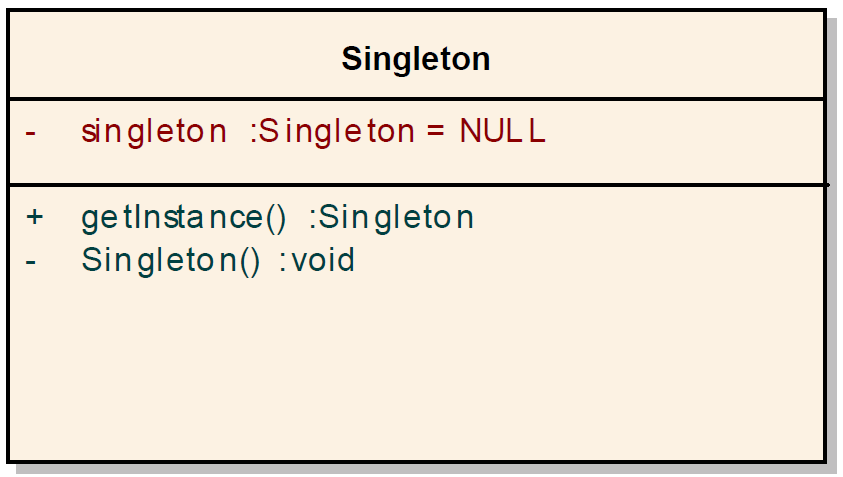
\includegraphics[width=0.6\linewidth]{figs/spm5/SingletonClass}
	\caption{En Singleton klasse}
	\label{fig:SingletonClass}
\end{figure}

\begin{itemize}
	\item Private constructor - Sikrer at kun klassen kan oprette en instans, ingen andre kan oprette eller kopiere den!
	\item statisk \textit{getInstance()} funktion - Statisk så den kan kaldes uden et objekt. Denne funktion returnerer instansen, og laver en ny hvis den private pointer (instansen) til sig selv er NULL.
	\item Statisk private pointer til sig selv - Den eneste instans\todo{right??}.
\end{itemize}

\subsubsection{Gof Observer Pattern}

\subsubsection{GoF Mediator Pattern}